\documentclass[12pt, letterpaper]{article}
\usepackage{graphicx}
\graphicspath{{images/}}
\title{MOSFET Current Source}
\author{}
\date{}
\begin{document}

\maketitle

\section*{Schematic}
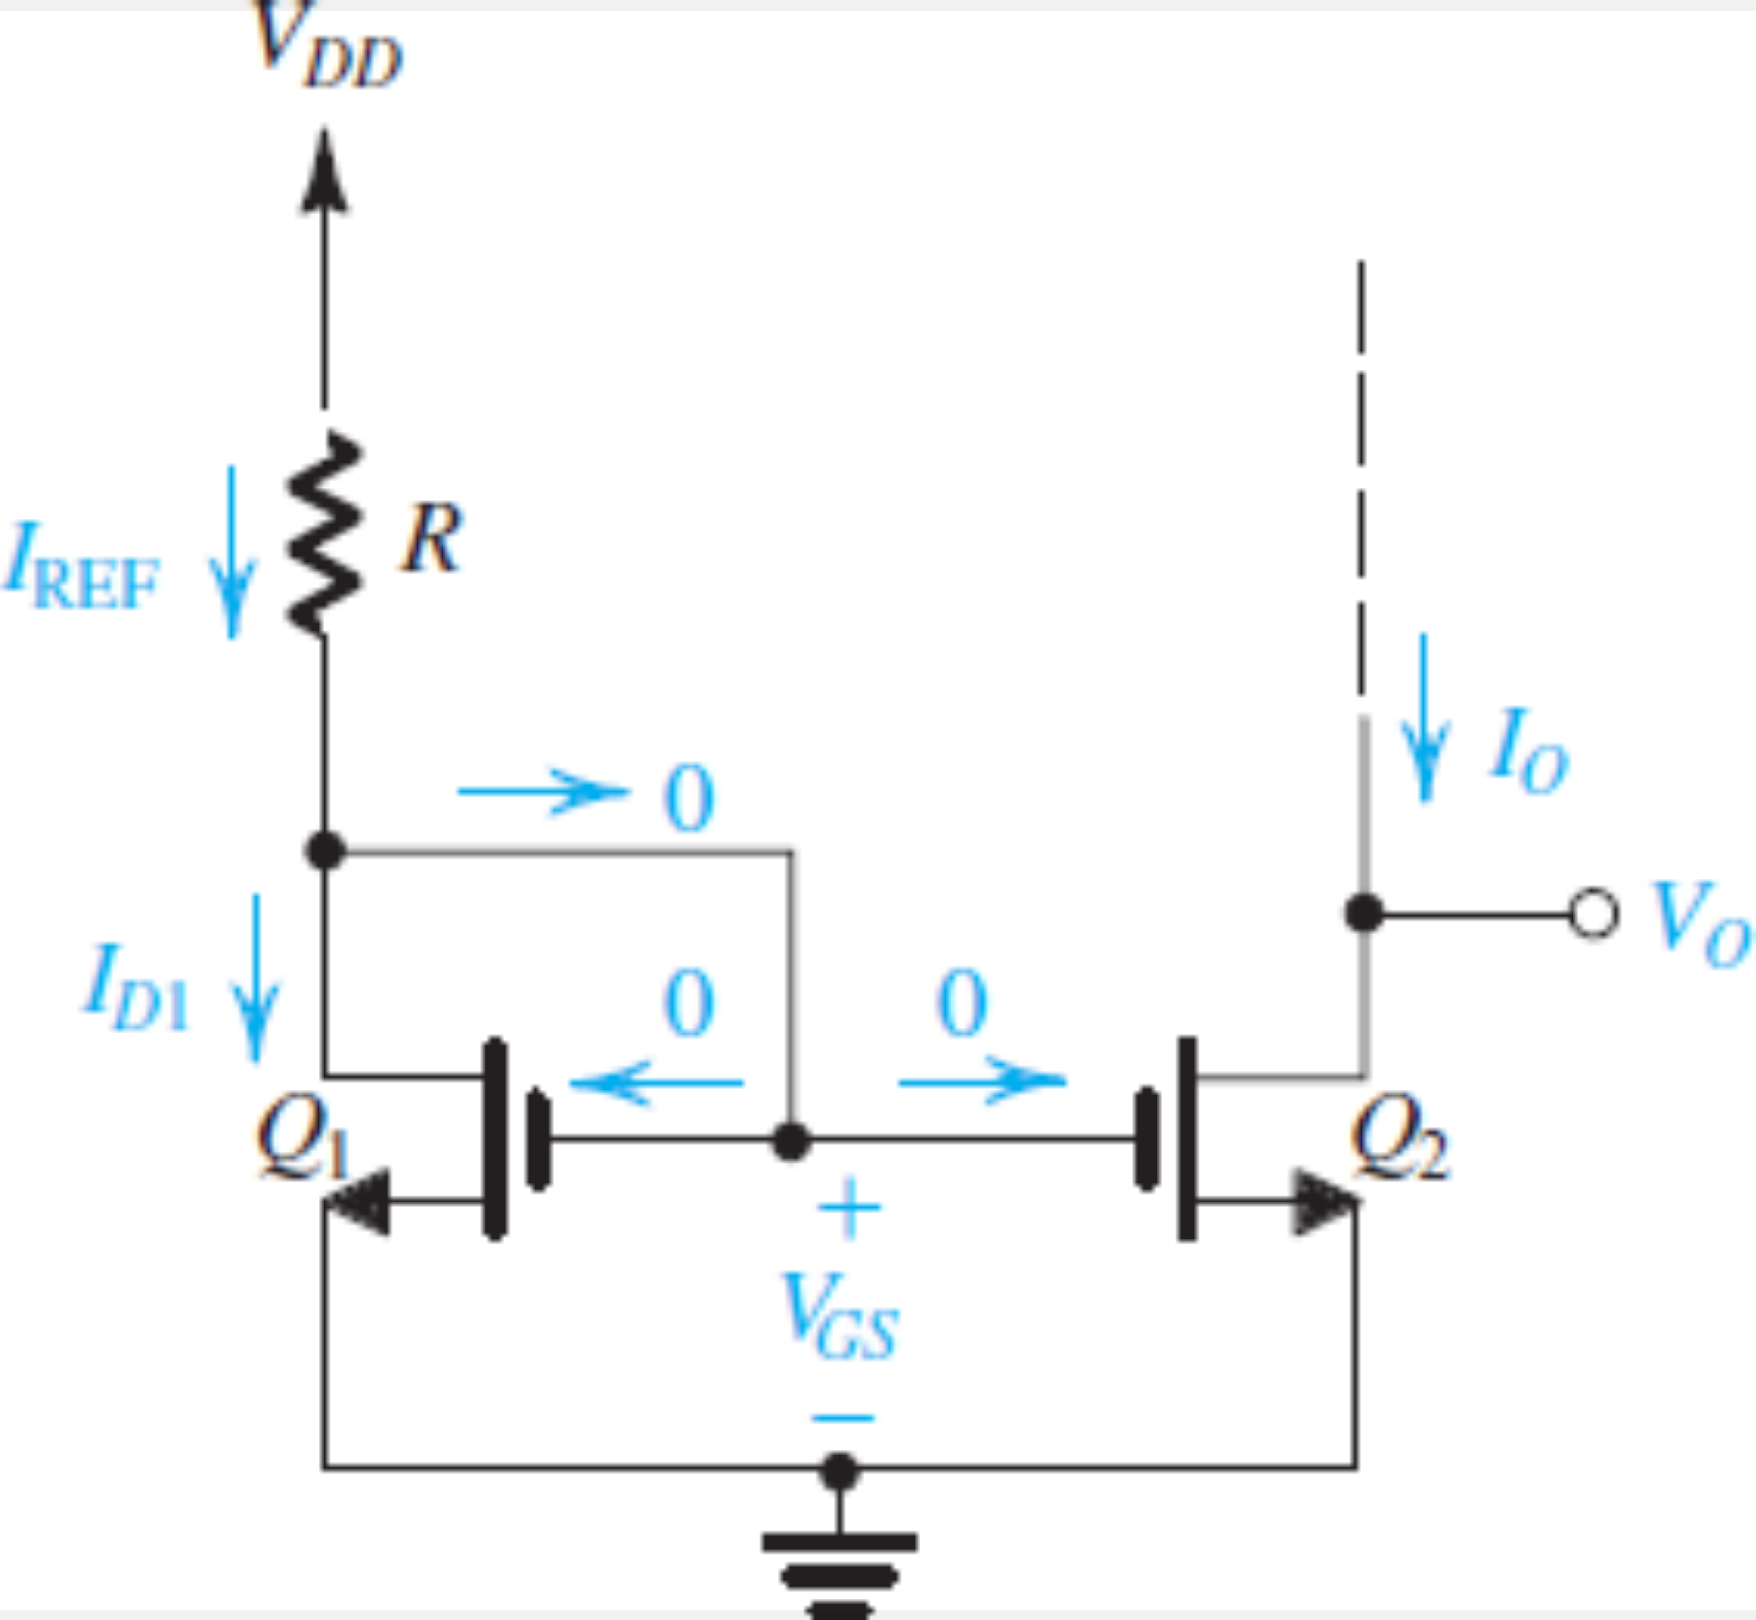
\includegraphics[width=0.95\linewidth]{current-source}
\subsection*{Small-Signal Model}
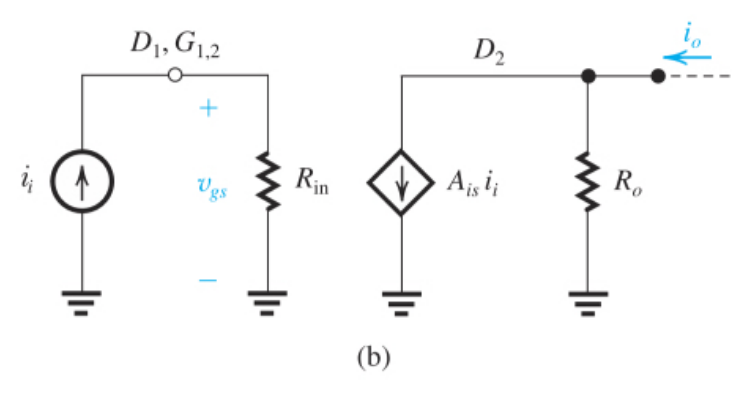
\includegraphics[width=0.95\linewidth]{small-signal}

\section*{Equations}
\begin{tabular}{ l l l }
Equation & Conditions & Notes \\ 
$I_{D1} = I_{REF} = \frac{V_{DD} - V_{GS}}{R}$ & & Gate currents are zero \\  
$I_O = I_{D2} = \frac{1}{2} k_n^{\prime} \left( \frac{W}{L} \right)_2 \left( V_{GS} - V_{t} \right)^2$ & $V_O \geq V_{GS} - V_t$ & Must operate in saturation region\\
$I_O = \frac{\left( W/L \right)_2}{\left( W/L \right)_1} I_{REF} \left[ 1 + \frac{V_O - V_{GS}}{V_{A2}} \right]$ & & \\
$\Delta I_O = \frac{\Delta V_O}{r_{o2}} = \frac{V_O - V_{GS}}{r_{o2}}$ & & \\
$\frac{I_O}{I_{REF}} = \frac{\left( W/L \right)_2}{\left( W/L \right)_1}$ & Negligible channel-length modulation & \\
$I_O = I_{REF}$ & Identical transistors & \\
$A_{is} = \frac{g_{m2}}{g_{m1}} \frac{1}{1 + \left( 1/{g_{m1} r_{o1}} \right)}$ & & \\
$A_{is} = \frac{\left( W/L \right)_2}{\left( W/L \right)_1} \left[ \frac{1}{1 + \left( 1/{g_{m1} r_{o1}} \right)} \right]$ & & \\
\end{tabular}

\section*{Notes}
\begin{tabular}{ l l }
Term & Description \\
$A_{is}$ & Small signal short-circuit current gain \\
\end{tabular}

\end{document}
